\part{Transposers}\label{part-2.-Transivitizers}

\chapter{Rhymes in early poetry}


Ode 18, stanza 1

\begin{tabular}{lll}
{\Large 羔羊之皮} & \textit{bie} & On the Lamb furs,   \\
{\Large 素絲五紽} & \textit{da} & five many-thread tresses of white silk;
\end{tabular}

Odes 145, stanza 1 

\begin{tabular}{lll}
{\Large 彼澤之陂} & \textit{pie} & By the shore of that marsh   \\
{\Large 有蒲與荷} & \textit{ḫa} & there are sedges and lotus
plants; 
\end{tabular}

So, -\textit{ie} and -\textit{a} rhymed in the Odes. 




\chapter{Tongjia 通假}

\chapter{Paronomastic glosses}

Shìmíng (c. 200) etc.


\chapter{讀若 dúruò}

Boltz 2017


\chapter{反切 fǎnqiè}
The pronunciation
of characters may be  presented using 反切 `\emph{fǎnqiè}. 
This method is traditionally credited to 孫炎 Sūn Yán
(220--280 CE) but perhaps used by the earlier scholars Yìng Shào 應劭
(140-206 CE) and 服虔 Fú Qián (late 2nd century) 
\citep[38]{Branner2000c}. The
 \emph{fǎnqiè} method represents a character's pronunciation by
giving two further characters; the first character shares the same onset
as the character annotated and the second character has the same rime as
the character annotated.\footnote{I use `onset' in this setting to
  indicate the phonetic quality shared by the reading of a character and
  the reading of the first of its two  \emph{fǎnqiè }spellers (反切上字
   \emph{fǎnqiè shǎngzì} hereafter `\emph{fǎnqiè} onset spellers'). As
  described below, assuming that the sameness of this relationship is
  transitive `onset' becomes equivalent to 聲類  \emph{shēnglèi}. I
  reserve `initial' for sets of `onsets' in complementary distribution.
  Although not equivalent `onset' is thus closer to an allophone whereas
  `initial' is closer to a phoneme.} To give a concrete example, the
character 東  \emph{tuwng} is glossed with 德 \emph{tok} and 紅
 \emph{huwng}, where the pro­nun­ci­a­tion \emph{tuwng} has the initial
of \emph{t}- of 德  \emph{tok} and the rime -\emph{uwng} of 紅
 \emph{huwng}; one can represent this relationship an equation: 東
 \emph{tuwng} = 德 \emph{t}(\emph{ok}) + 紅 (\emph{h})\emph{uwng}. The
analysis of the pro­nun­ci­a­tion of `fake' as \emph{f}(\emph{old}) +
(\emph{c})\emph{ake}, is an analogous use of the  \emph{fǎnqiè} method in
English.


as early as 2nd century, but more complete in

\subsection{Yùpiān (544)}

\subsection{Jīngdiăn shìwén (582-589)}

\subsection{Qièyùn 切韻  (602) and derivative works}

\paragraph{The `ranks' of the rime tables.} Without explanation the rime tables
classify rimes among four 等~ \emph{děng} `ranks'.\footnote{In English it is useful to distinguish between `rank' as
the term for the four rows of the rime tables and `division' for the
analogous but distinct categories in the  \emph{Qièyùn}, even though the
Chinese term 等~ \emph{děng} is the same in both cases 
\citep[13]{Shen2017}.}
These `ranks' refer
fundamentally to the \emph{mise-en-page} of these two particular
documents, each rank corresponding to a row on a page. Although the
linguistic meaning of these `ranks' is obscure, they bear certain
relationships with dis­tri­bu­tional classes of co-occurrences between
initials and rimes in the \emph{Qièyùn} (\cite[7]{Schuessler2009minimal}, 
\cite[]{Shen2017}). 



\begin{figure}[htbp]
    \centering
    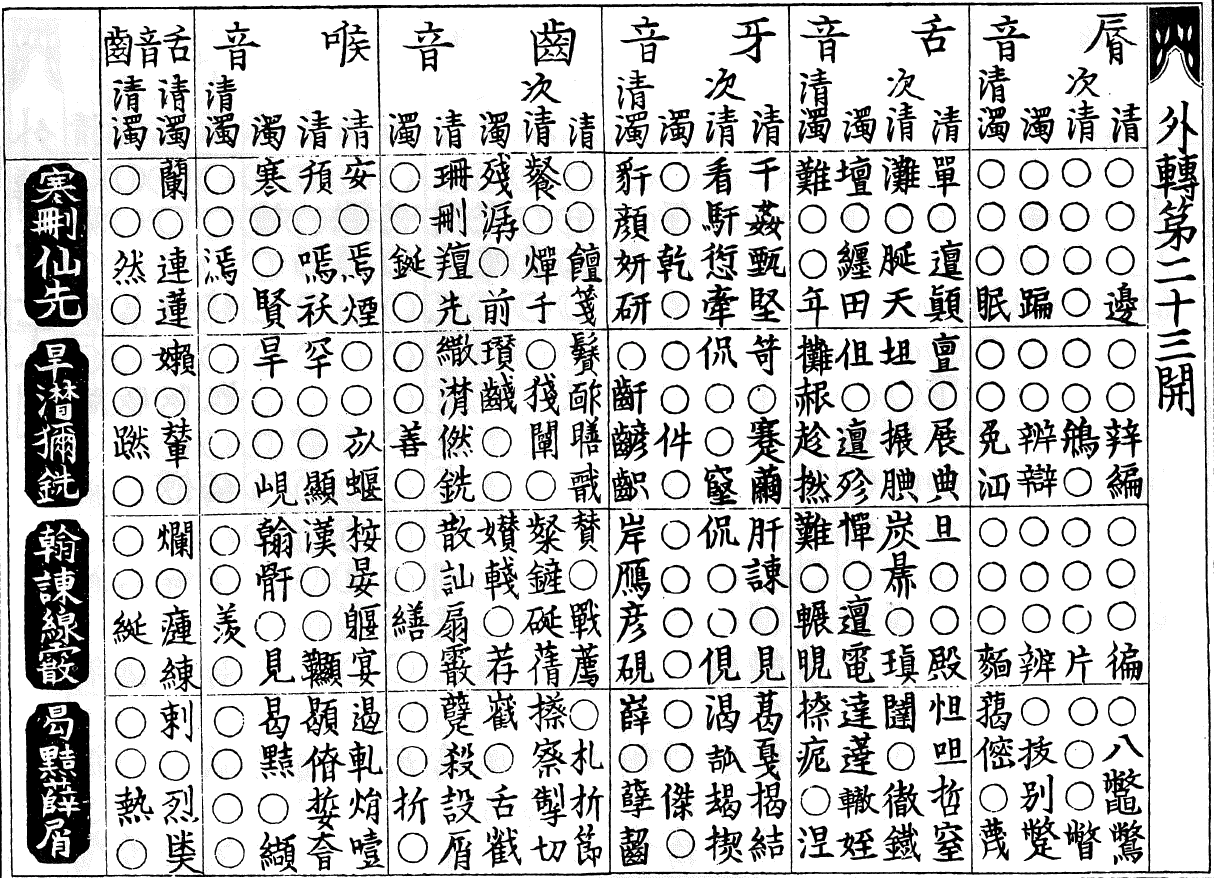
\includegraphics[width=1\textwidth]{Chapter5/fig17 Yunjing 23 version 1.png}
    \caption{Chart 23 from the \textit{Yùnjìng}}
    \label{fig:Yunjing23}
\end{figure}

\begin{figure}[htbp]
    \centering
    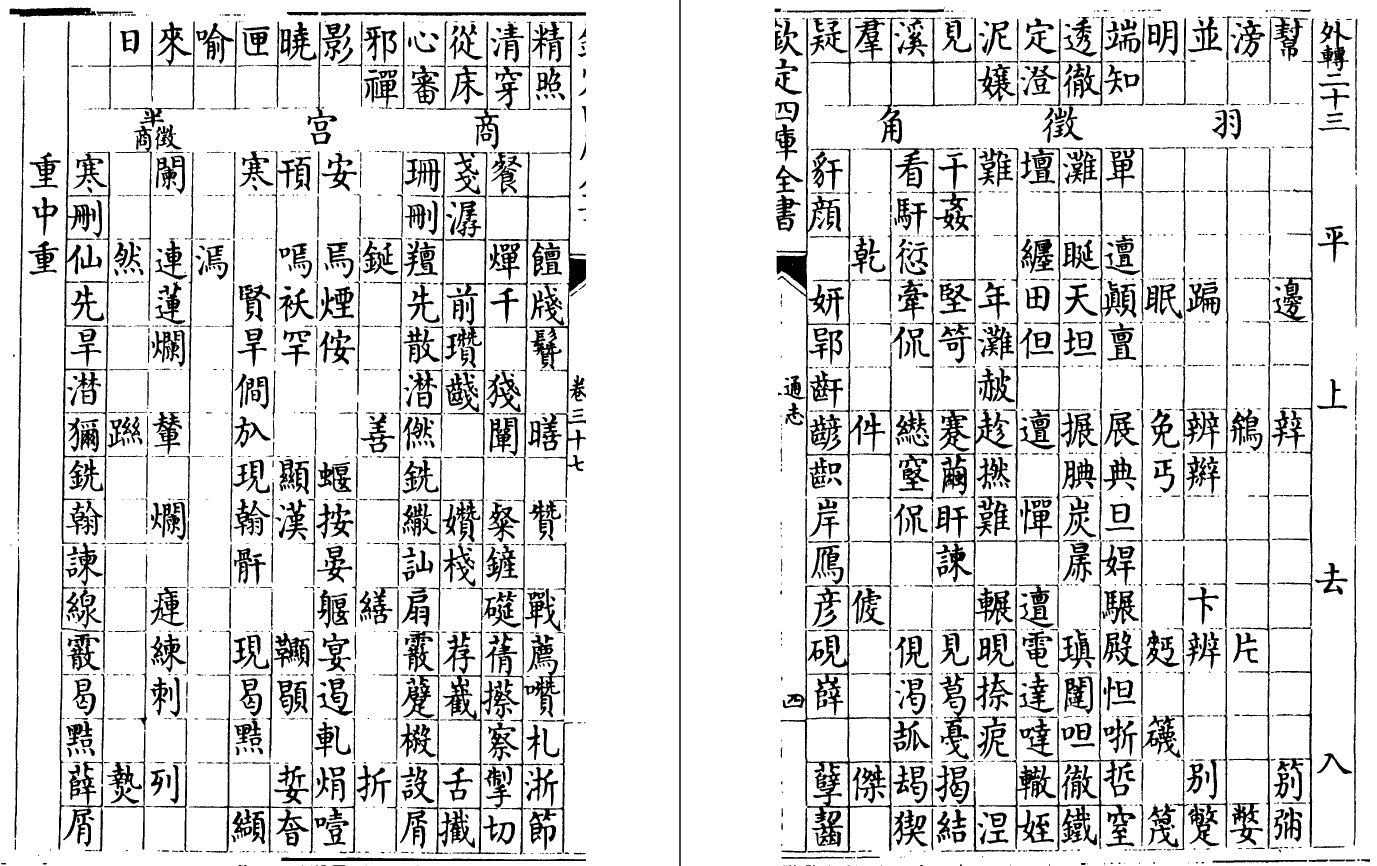
\includegraphics[width=1\textwidth]{Chapter5/fig18 Qiyinlue 23 version 1.png}
    \caption{Chart 23 from the \textit{Qīyīnlüè}}
    \label{fig:Qinyinlue23}
\end{figure}


